\subsubsection{Navigation Flow Diagram}

The Navigation Flow Diagram illustrates the sequences through which users can access the application's different screens to complete their tasks. Below, the application's navigation flow diagram is shown in Figure \ref{fig:navigation-flow-diagram}.

\begin{figure}[H]
    \centering
    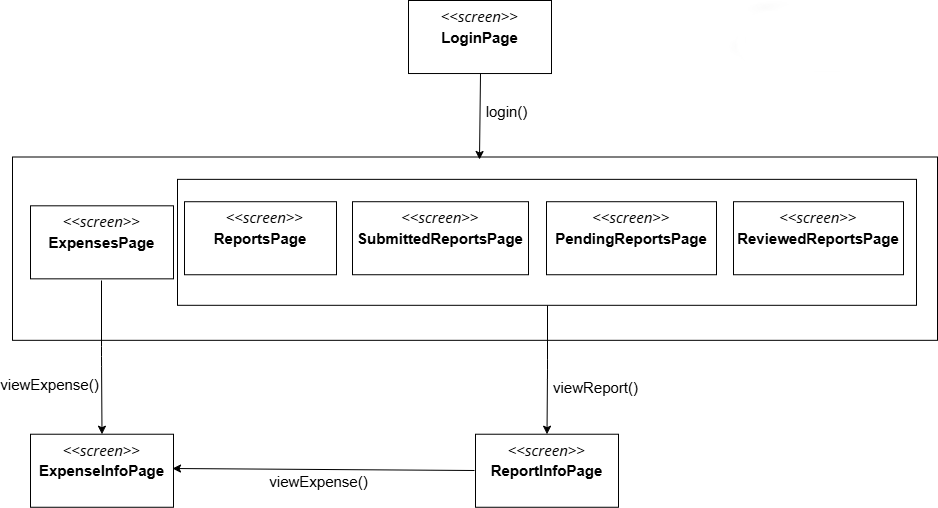
\includegraphics[width=\textwidth]{Images/NavigationFlowDiagram.png}
    \caption[Navigation flow diagram]
    {Navigation flow diagram. [Own creation]}
    \label{fig:navigation-flow-diagram}
\end{figure}

The overall navigation flow is designed to be logical and task-oriented, guiding users through the application's functionalities. Each time a user accesses the application, the LoginPage is displayed, requiring authentication via a corporate email address. Upon successful authentication, the user is redirected to the default ExpensesPage. However, users may freely navigate to other main screens. Each main screen corresponds to a functional area described in Section \ref{sec:functional-areas}, where users can perform the tasks outlined in the use case diagrams from the same section.

The application's main screens are defined as follows:

\begin{itemize} [leftmargin=0.75cm, label=\textbullet, noitemsep]

    \item \textbf{ExpensesPage}: Displays all expenses uploaded by the user that are not yet associated with any report.

    \item \textbf{ReportsPage}: Displays all reports created by the user that have not yet been submitted for review.

    \item \textbf{SubmittedReportsPage}: Displays all reports created by the user that have been submitted to a reviewer.

    \item \textbf{PendingReportsPage}: Accessible only to Admin users; displays all reports submitted to the Admin that are pending review.

    \item \textbf{ReviewerReportsPage}: Accessible only to Admin users; displays all reports that have been submitted to and reviewed by the Admin.

\end{itemize}

From any main screen, users can select an expense or report and navigate to the corresponding \textbf{ExpenseInfoPage or ReportInfoPage} to view detailed information. Within the ReportInfoPage, a list of associated expenses is presented, allowing users to further navigate to the respective \textbf{ExpenseInfoPage} entries.

Both \textbf{ReportInfoPage} and \textbf{ExpenseInfoPage} enable users to view detailed information and, when permitted, edit the displayed data. These pages remain editable only while the report has not been submitted. When accessed from \textbf{SubmittedReportsPage}, \textbf{PendingReportsPage}, or \textbf{ReviewerReportsPage}, both pages are presented in a read-only state.

As described in Section \ref{sec:logical-architecture}, the user interface follows a component-based architecture, where each component is constructed using reusable elements. This approach facilitates a consistent and simplified navigation flow. The \textbf{ExpensesPage} design is reused across other main report-related screens, which also share the same \textbf{ReportInfoPage}. Similarly, the \textbf{ExpenseInfoPage} is reused across both \textbf{ExpensesPage} and \textbf{ReportInfoPage}.
